This project represents the physical adaptation of an autonomous landing solution developed in simulation in \cite{AL_thesis}. The first phase of software development in this project was the adaptation of this software from the simulation environment to the physical drone system.

\begin{figure}
    \centering
    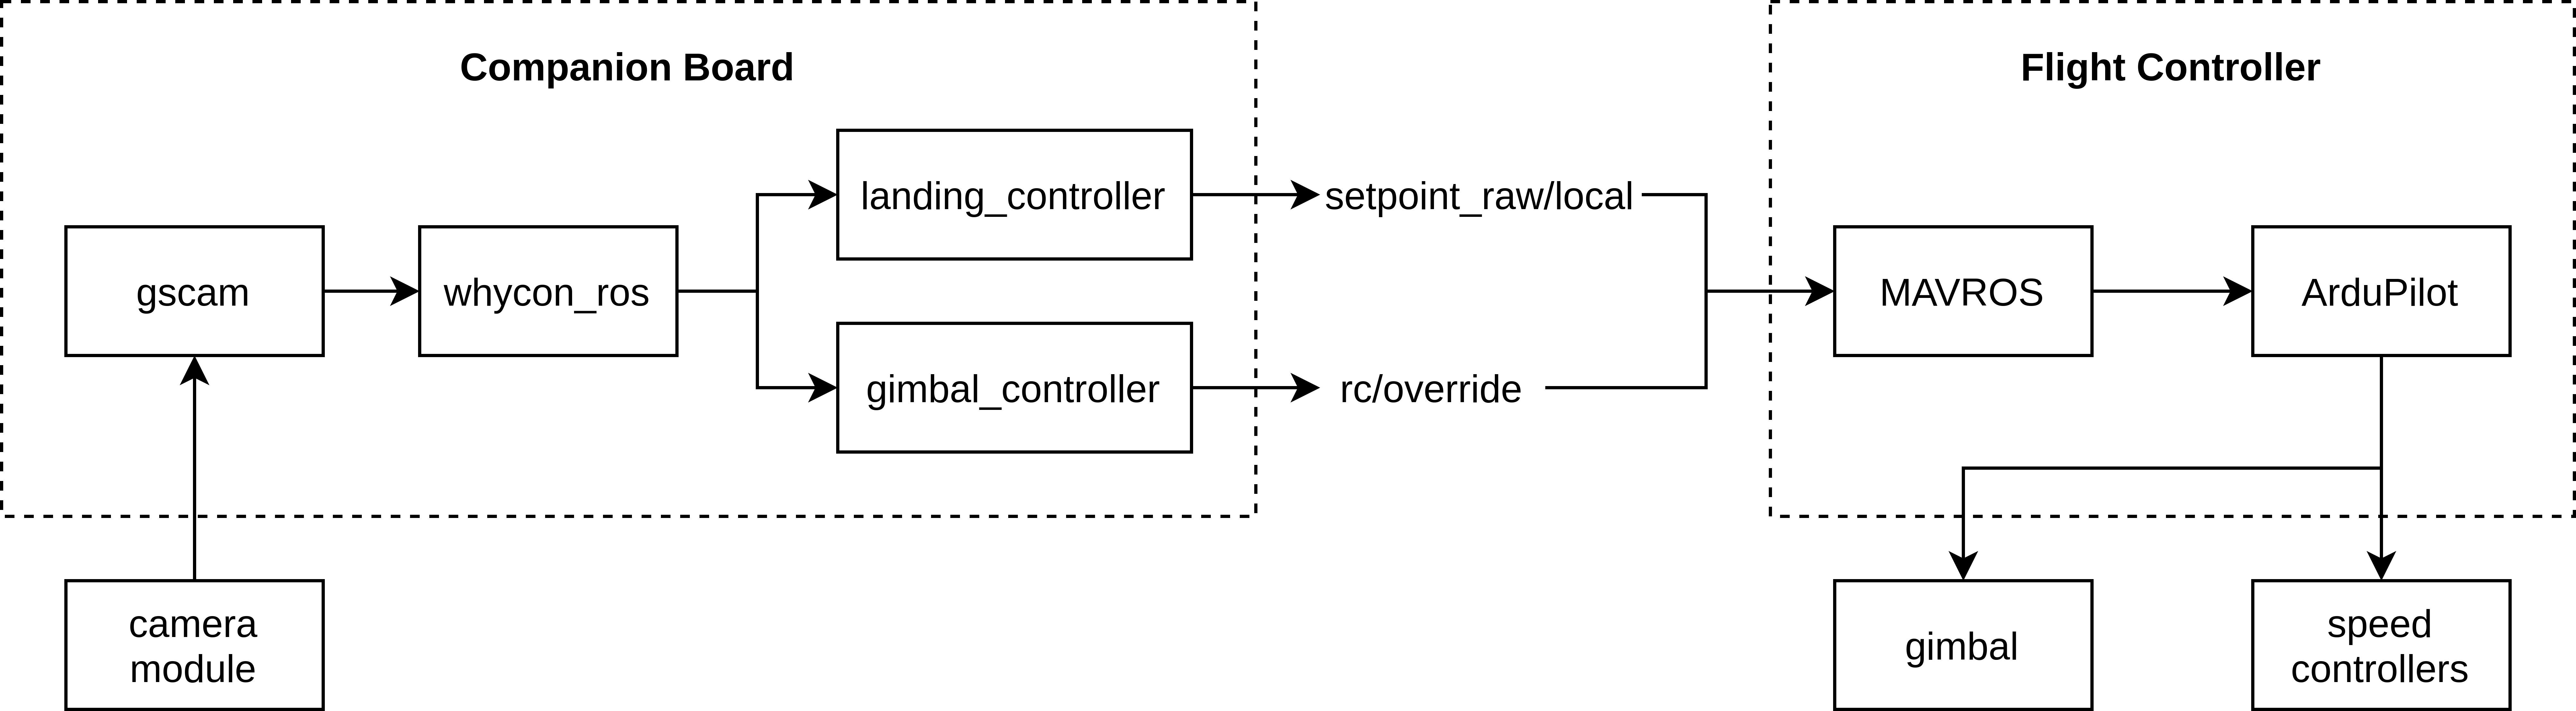
\includegraphics[width=\textwidth]{images/data_flow.png}
    \caption{Data flow.}
    \label{fig:data_flow}
\end{figure}

\subsubsection{Video Input Processing}

The Gazebo simulator in which this software was originally tested and developed provides simulated camera modules which natively provide images as a ROS topic. Joshua and Kjartan replicated this functionality with physical camera modules. This was done with a ROS package called \texttt{gscam} \cite{gscam_github}, which is designed for this functionality and acts as an interface between GStreamer (a tool for manipulating video and music files) \cite{gstreamer_website} and ROS. On the Google Coral, this was accomplished simply by using the \texttt{gscam} module alone, and on the NVIDIA Jetson Nano, this was accomplished using \texttt{gscam} and an extension to it which is called \texttt{jetson\_csi\_cam} \cite{jetson_csi_cam_github}. The \texttt{gscam} works with GStreamer pipelines, which allow simple video manipulation such as rotation and resizing, and ultimately stream the image to ROS as an image topic.

Initial tests shows an extremely high computation load and low framerate when identifying a WhyCon marker from the camera stream at full resolution. In order to reduce the computational requirements of the video analysis, the video stream is first resized by GStreamer to a manageable 640x480 resolution, from the native resolutions of 3280x2464 and 2582x1933 for the Jetson and Coral camera modules respectively. The 640x480 resolution allowed the video to be analyzed at about 30 frames per second, however this parameter is not necessarily optimal and could be changed in the future. It provided a significant performance boost over the native resolutions which allowed only a very slow analysis framerate. In the earlier revisions of the camera module cases, the video was also rotated to the correct orientation using the GStreamer pipeline before analysis.

The camera's intrinsic matrix and distortion coefficients were found through the typical ``chessboard'' calibration method using the ROS \texttt{camera\_calibration} module \cite{ros_camera_calibration} which is outlined in the original thesis \cite{AL_thesis}. The Google Coral's camera module has significantly less distortion than the Jetson Nano's wide-angle camera module because of its smaller field of view (84\degree vertically and 87.6\degree horizontally). The Jetson Nano's camera module has a field of view of 160\degree diagonally. Its large field of view makes it easier to detect fiducial markers at close range.

\subsubsection{WhyCon Adaptation}
\label{section:whycon_adaptation}

The original landing software, tested in simulation, used both April Tag and WhyCon fiducial markers, but only WhyCon is used on the physical systems in order to reduce computational load on the companion board. For context, the April Tag module was only added for reliable estimation of the yaw (rotation in the z-axis) of the landing platform, as there is some issue in determining the yaw orientation of WhyCode markers (outlined in the original thesis \cite{AL_thesis}). 

The \texttt{whycon\_ros} module from LCAS \cite{whycon_github} was only slightly modified for use in this project, and the modifications are listed below:

First, the pixel positions $u,v$ for the center of the marker were populated as part of the WhyCon/Marker message. The $u \in [0, 640]$ corresponds to the marker's $x$ position in the resized camera frame, and $v \in [0, 480]$ corresponds to the marker's $y$ position in the resized camera frame. These pixel positions allow the gimbal controller to aim the camera directly at the marker with fewer calculations than in the original software, since the pixel offset of the marker from the center of the camera's field of view corresponds roughly to physical angle offset between the marker's position and the camera's rotation in space.

Second, an additional message attribute called \texttt{theta}, in the message definition, (hereafter referred to as $\theta$) describes the $z$-axis rotation of the marker in space according to the pixel placement of its white and black regions. The centers of the white and black regions are not published as topics by the module, but they are used in other calculations and are therefore easily available in the code. If the black segment has center $u_b,v_b$ and the white segment has center $u_w,v_w$, then $\theta$ is calculated as follows:

$$\theta_i = arctan\left(\frac{v_w - v_b}{u_w - u_b}\right)$$
$$\theta = \begin{cases}
    \theta_i + \frac{\pi}{2} &\mbox{if } \theta_i \leq \frac{\pi}{2} \\
    \theta_i - \frac{3\pi}{2} &\mbox{if } \theta_i > \frac{\pi}{2}
\end{cases}$$

Then $\theta$ is the angle from the center of the marker to the center of its white region. This helps to reduce some confusion that results from rotationally symmetric markers, such as 2-bit WhyCode markers with IDs 1 and 2, shown in Figures \ref{fig:whycode_1} and \ref{fig:whycode_2}, in that orients the marker with respect to the extended white region. In Figure \ref{fig:whycode_1}, $\theta = -\frac{\pi}{2}$, and in Figure \ref{fig:whycode_2}, $\theta = \frac{\pi}{2}$. This provides a reliable yaw orientation value for the marker, but ultimately did not solve the issue discussed in Section 3.3.1 of the original thesis \cite{AL_thesis}. 

\begin{figure}
    \centering
    \begin{subfigure}[b]{0.3\textwidth}
        \centering
        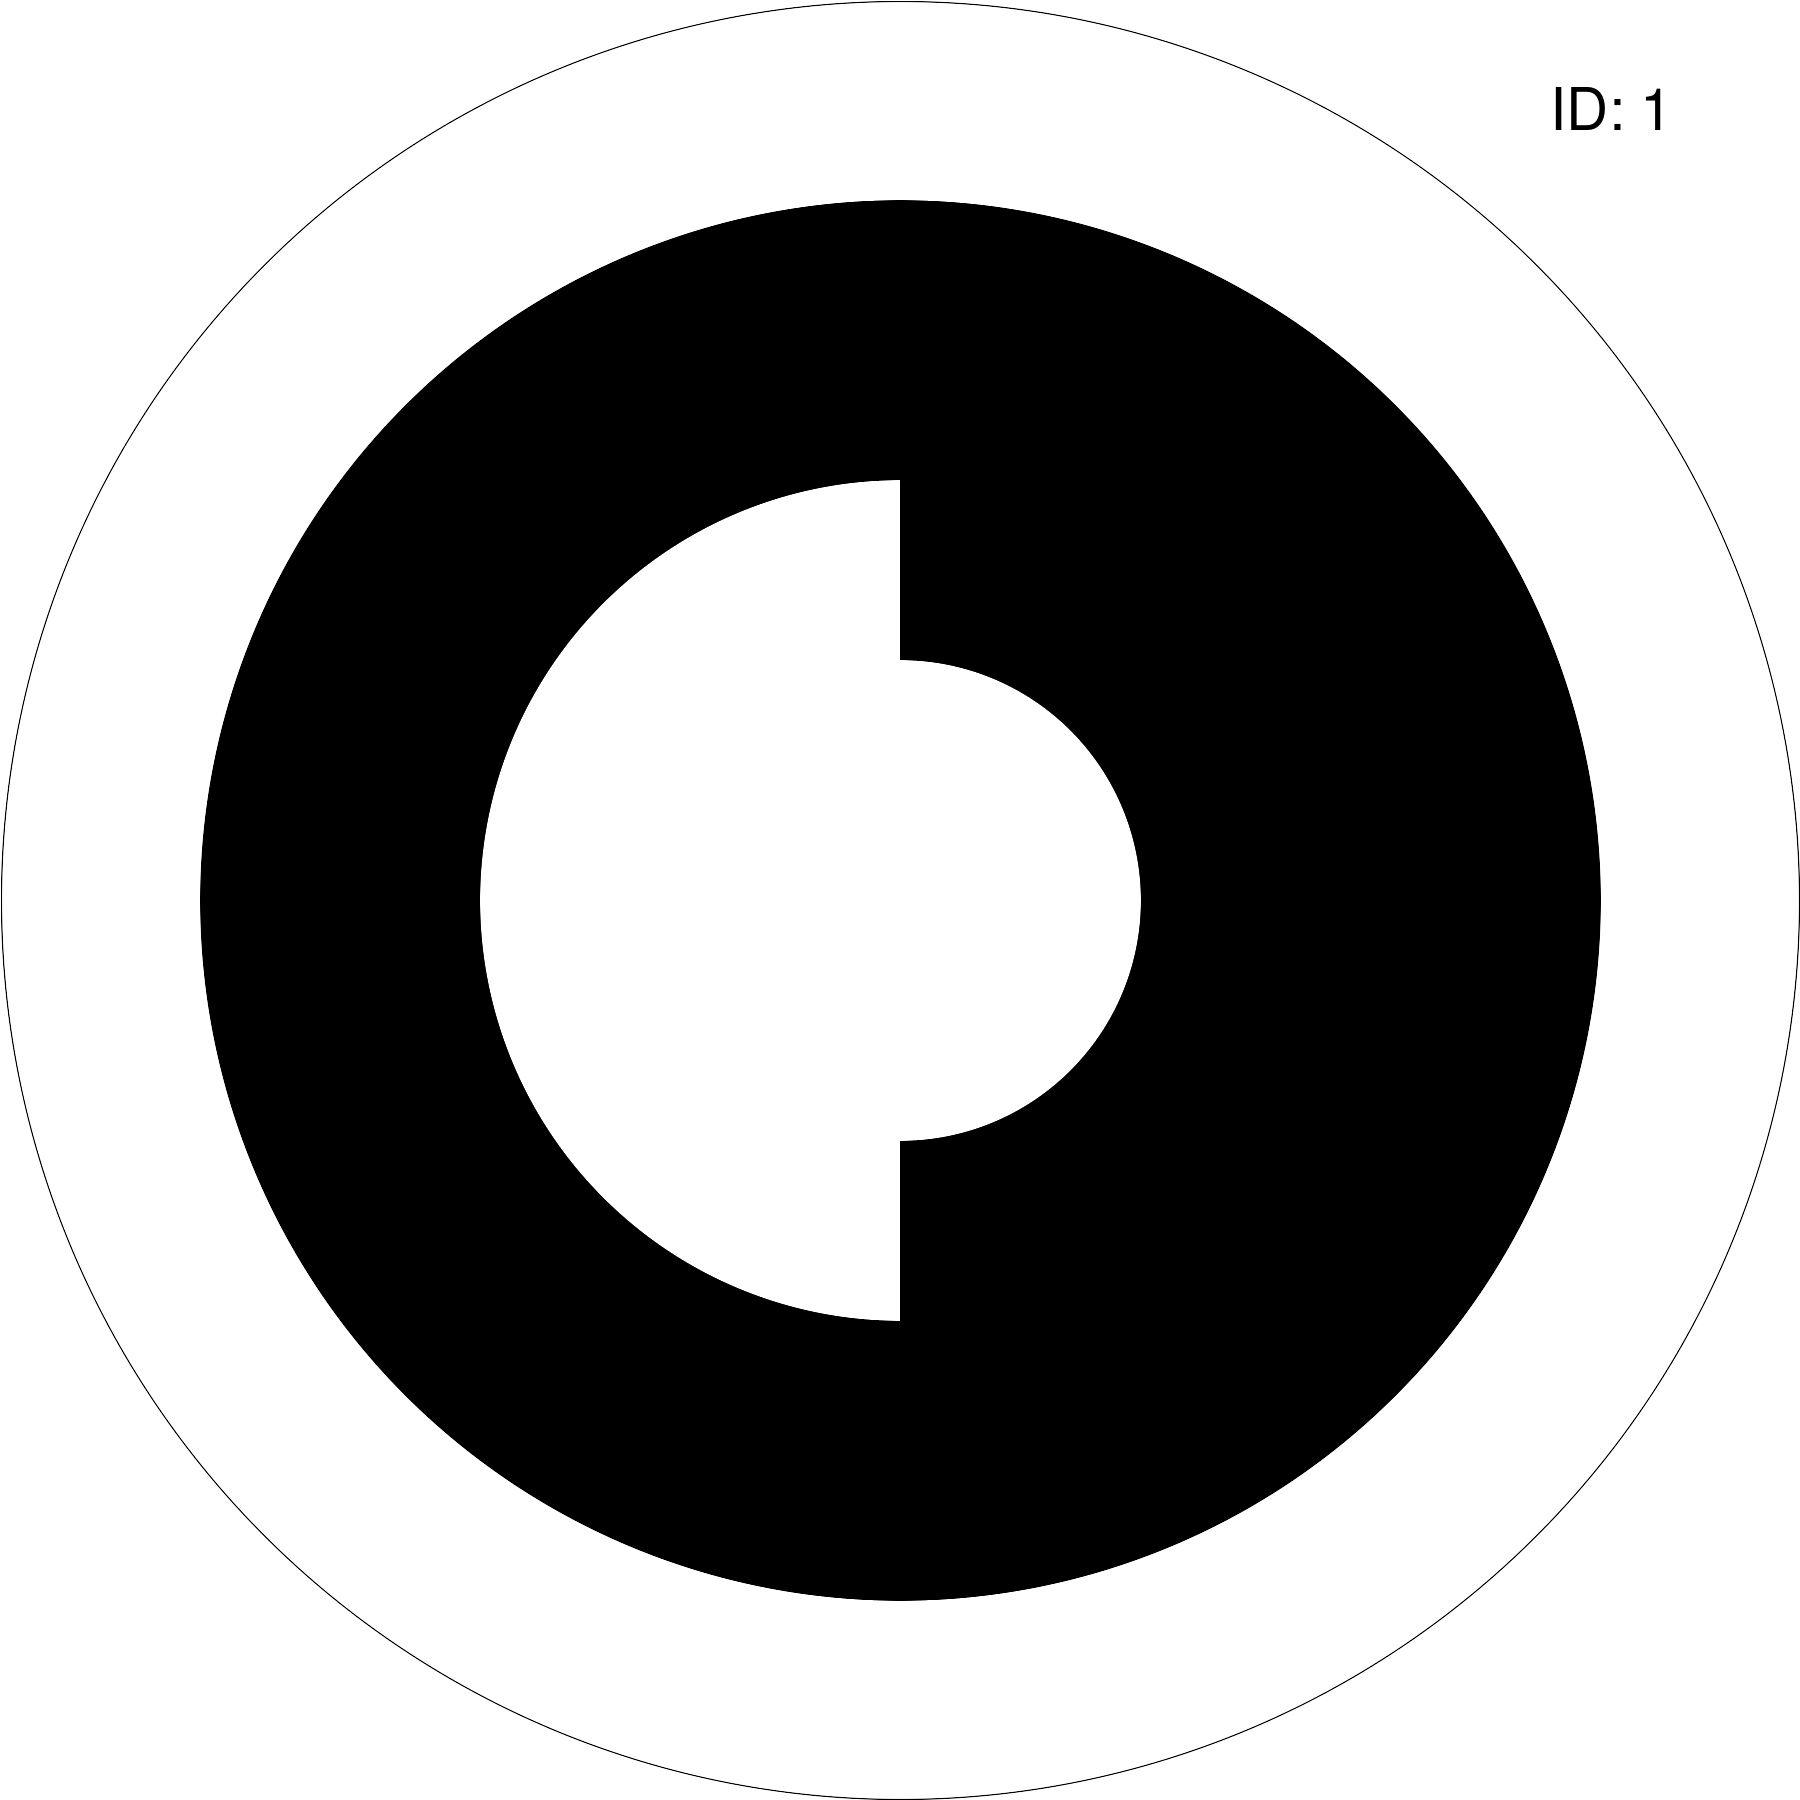
\includegraphics[width=\textwidth]{images/00000001.png}
        \caption{ID: 1}
        \label{fig:whycode_1}
    \end{subfigure}
    \begin{subfigure}[b]{0.3\textwidth}
        \centering
        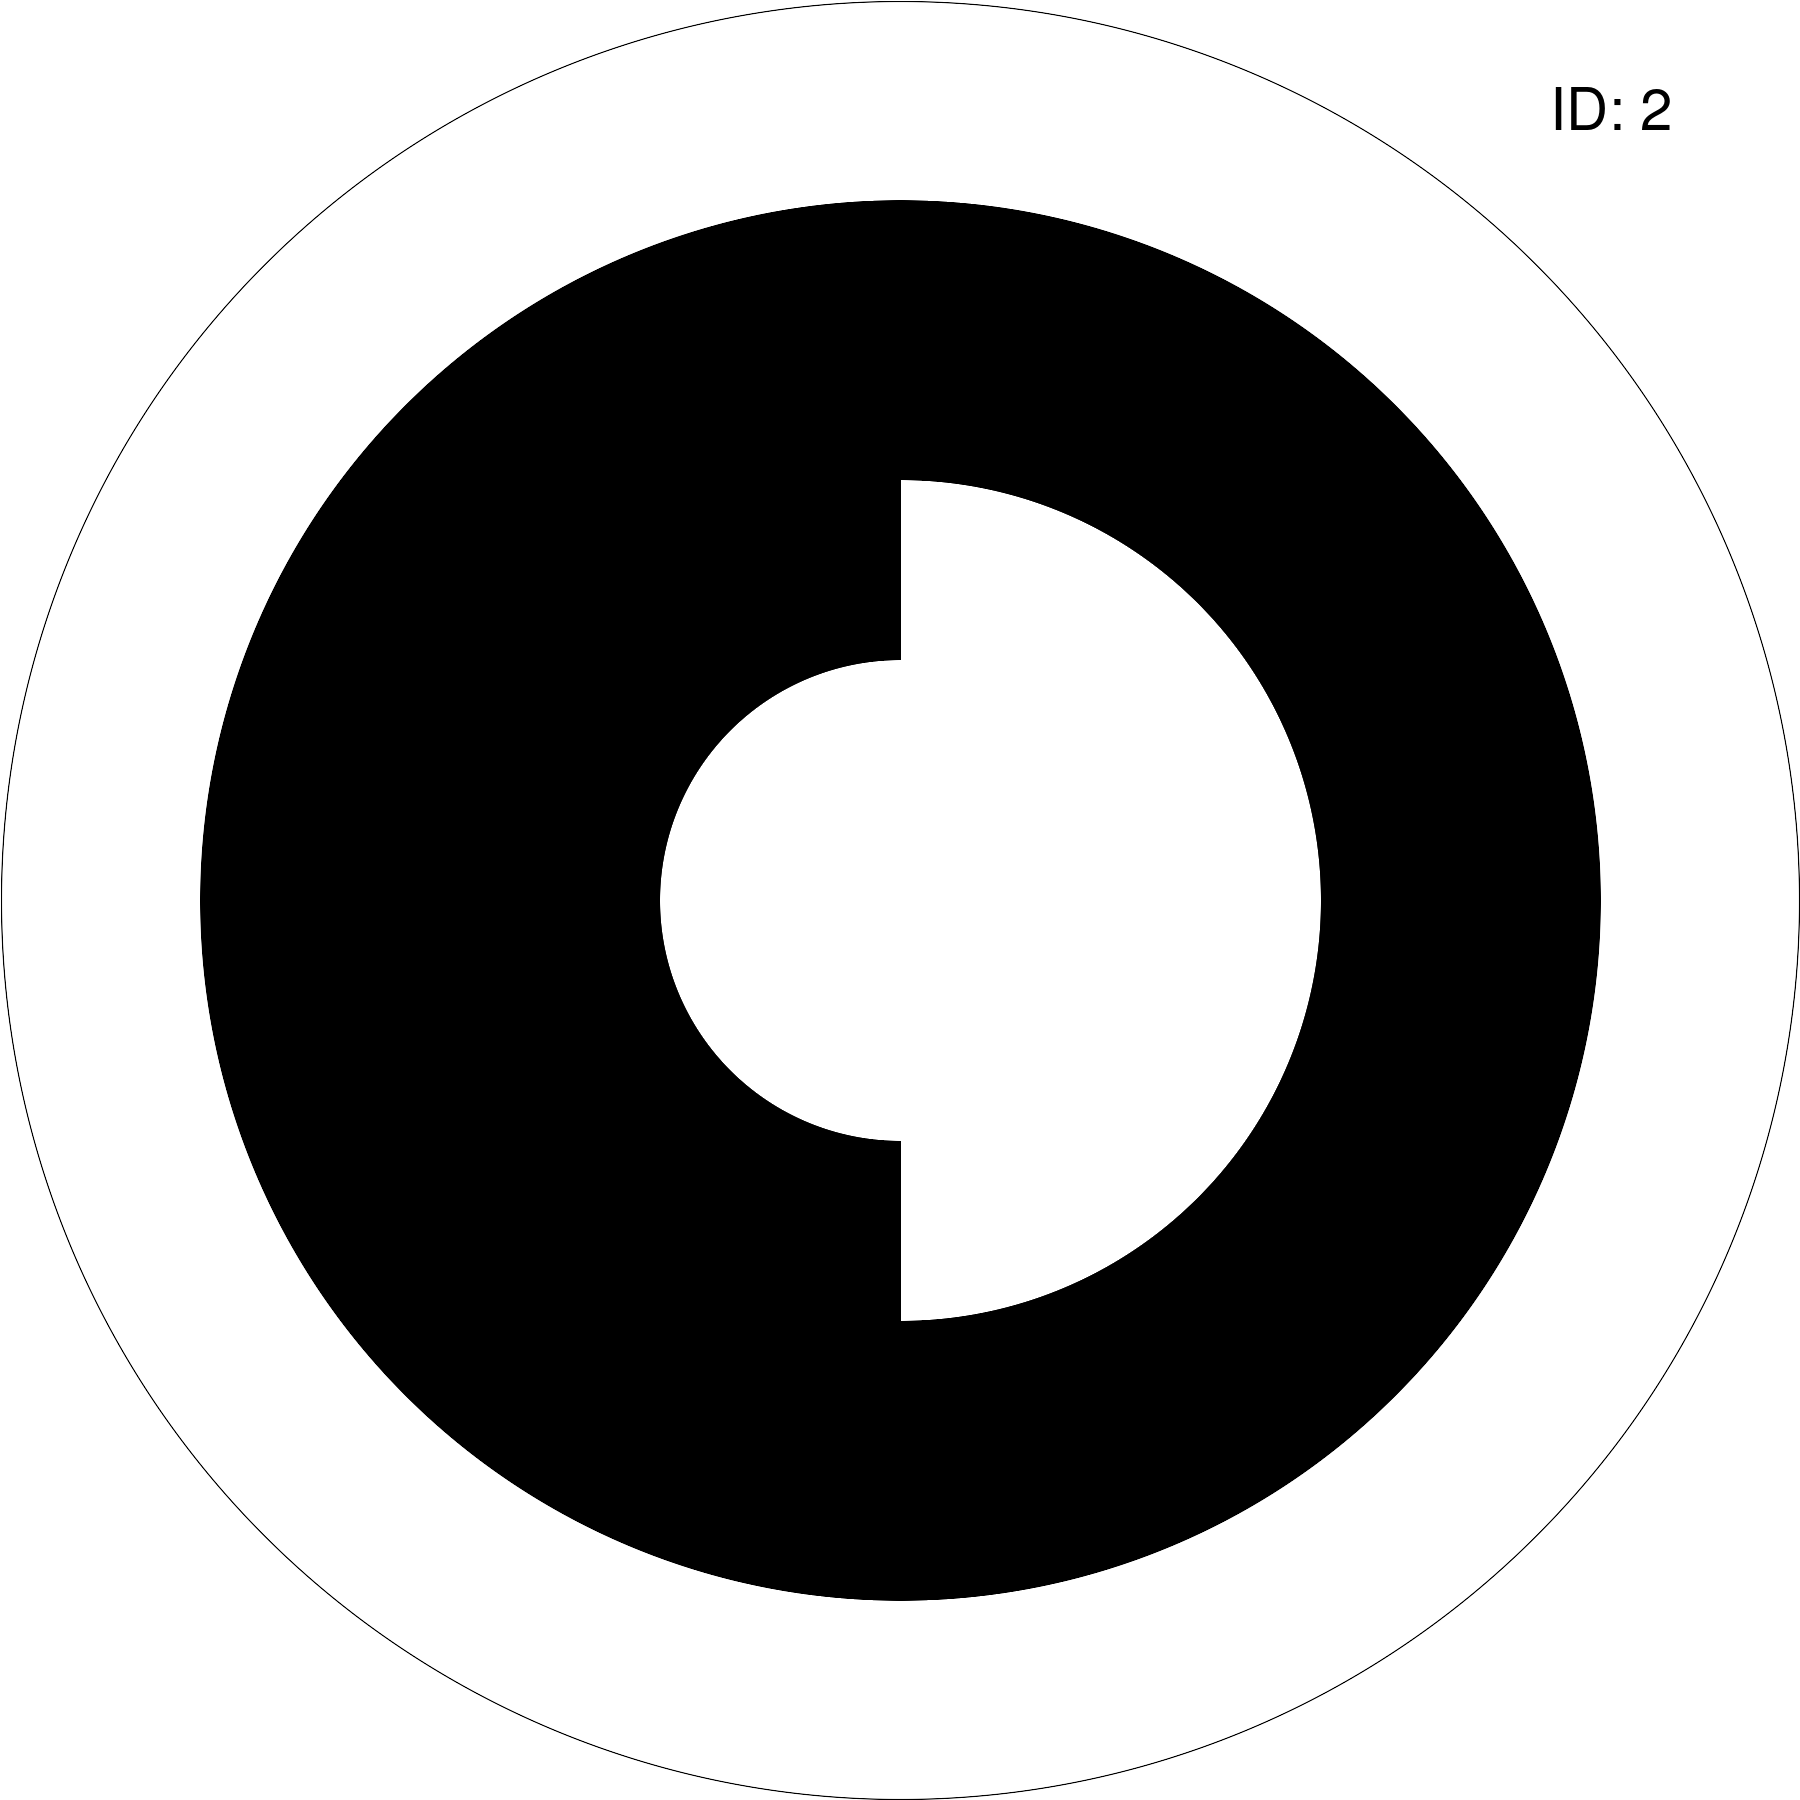
\includegraphics[width=\textwidth]{images/00000002.png}
        \caption{ID: 2}
        \label{fig:whycode_2}
    \end{subfigure}
    \caption{Rotationally symmetric WhyCode markers.}
    \label{fig:rotationally_symmetric WhyCode markers.}
\end{figure}

\subsubsection{Gimbal Controller Adaptation}
\label{section:gimbal_controller_adapation}
The gimbal controller ROS module \cite{gimbal_controller_github} has been simplified from the original simulation-tested code, in order to account for a simplified fiducial marker system. The original fiducial marker system included both a WhyCon and April Tag marker. However, in lab testing, running both fiducial systems was excessively processor intensive, typically requiring more than 50\% of CPU time, and so the April Tag marker was abandoned. The WhyCon marker alone used required less than 10\% of CPU time, although further analysis was outside the scope of this project. Overall, the purpose of the gimbal controller is to center the WhyCon marker in the camera frame by changing the pan and tilt angles of the gimbal using the pixel coordinates $u,v$ of the detected WhyCon marker.

PID controllers provide a simple means of smoothly controlling actuators.\cite{pid_control} Two PID controllers generate control effort signals which determine the rotation of the gimbal in its two axes. They take as state inputs the normalized values of $u,v$ which are $u_n, v_n \in [-1,1]$ and both have constant set points (target state values) of 0. They generate control efforts in the interval $[-1, 1]$, which are then converted to pulse width modulation (PWM) signals. These are standard signals for servo control. The gimbal controller module sends these PWM signals to ArduPilot via the MAVROS OverrideRCIn topic, and the flight controller generates the actual PWM signals on its servo output rail, controlling the gimbal.

One of the challenges in using this setup is that the true angle of the gimbal is not known, as the gimbal does not expose this information. The angles are estimated based on the known minimum and maximum angles of the gimbal which can be set in firmware. The angles can be estimated through linear interpolation from the control effort PWM signal to the angular range of the gimbal in some axis. Using, for example, the pan axis: if the control effort PWM signal is $\mathrm{PWM}_\mathrm{pan} \in [1000, 2000]$, and the pan angle $\theta_\mathrm{pan} \in [-30, 30]$, then $\theta_{pan}$ is calculated as in Equation \eqref{equation:theta_pan}:

\begin{equation}
    \theta_\mathrm{pan} = -30 + \frac{(\mathrm{PWM}_\mathrm{tilt} - 1000)(2000 - 1000)}{30 - (-30)}
    \label{equation:theta_pan}
\end{equation}

This is only an estimate of the pan angle because the gimbal controller itself implements PID controllers in all of its axes, meaning that the angle of the gimbal does not directly correspond to the control signal when the entire gimbal is turning relative to its tilt axis. This happens when the drone has some non-zero yaw velocity. We reduced this effect by commanding the drone to maintain its yaw position throughout the course of landing.

\subsubsection{Landing Controller Adaptation} 

The purpose of the landing controller ROS module \cite{landing_controller_github} is to use the information from the gimbal controller to direct the drone towards the landing pad. Joshua adapted the landing controller from the original version, which uses velocity targets, to a simpler version using positional targets. The landing controller uses the estimated relative pose of the landing pad's WhyCon marker as a positional target. In order to calculate the positional target, the landing controller transforms the WhyCon marker's relative pose using transforms generated by the gimbal controller, which take into account the 2-dimensional rotation (in the pitch and roll axes) as well as the yaw of the gimbal.  When the landing controller detects that the drone is in "GUIDED" mode and the motors are armed, then the landing controller is enabled and publishes positional targets to the \texttt{setpoint\_raw/local} topic of MAVROS, which then relays the positional target to ArduPilot. The positional target is the 3-dimensional displacement of the drone from the landing pad. It also has a positional offset in the ``north'' (front) axis, meaning that the drone should land not directly on top of the marker, but rather offset slightly in one direction. This allows the drone to track the marker throughout its entire descent because the camera never gets prohibitively close to the marker, so the marker always fits in the camera's field of view. Similar projects have attempted to land directly on top of the marker, which causes the marker to exceed the camera's field of view and close distances and become undetectable. Since the WhyCon marker has no inherent yaw orientation, no target yaw of the drone is considered. This means that the drone can land around the landing pad with a radius determined by its target positional offset in the north axis. Landing on a radius around the landing pad, instead of on a specific point, is not ideal. In future work, a WhyCode marker will be used. This is a necessary first step due to limitations on detecting the yaw of WhyCode markers, which is discussed in Section 3.3.1 of the original thesis \cite{AL_thesis}.